 %++++++++++++++++++++++++++++++++++++++++
\documentclass[letterpaper,12pt]{article}
\usepackage{tabularx} 
\usepackage{amsmath}  
\usepackage{graphicx} 
\usepackage[margin=1in,letterpaper]{geometry} 
\usepackage{cite} 
\usepackage[final]{hyperref} 
\hypersetup{
    colorlinks=true,     
    linkcolor=blue,      
    citecolor=blue,        
    filecolor=magenta,     
    urlcolor=blue         
}
%++++++++++++++++++++++++++++++++++++++++


\begin{document}

\title{A Brief Exploration of the NBA Draft}
\author{Mike "dirty-mike" Neuder}
\date{\today}
\maketitle

\begin{abstract}
This quick analysis of the NBA draft was inspired and written for Phil Derbesy and Michael Chiappini of the exceptional podcast, "The Basketball Guyaries". During Episode 4, they are exploring the complexity of the current NBA draft, and ask for a bit of clarification on the probabilities going on to determine the order of picks. With the 2017 Draft just occurring, it seemed appropriate to take a glance at the process and learn more about how 14 ping-pong balls can change everything.
\end{abstract}

\section{Current Lottery System}
The current weighted lottery system was implemented in 1990 and reformed in 1993. The system was changed due to teams allegedly losing games intentionally during the near the end of the season in order to secure the first pick in the draft, as the team with the worst record of the season got the first pick. In the new weighted lottery system, the teams with the worst records still have the highest chance to pick early in the draft, however there is an element of randomness introduced in order to make it less appealing to be the worst team in the NBA. Currently, with 30 teams in the NBA, 16 will qualify for the playoffs and the remaining 14 are eligible to participate in the lottery. Since 1987, only the first three picks are determined by the lottery, and the remaining picks are done in reverse record order. Under this current system, the worst team of the previous season at least would be picking fourth in the draft, while the second worst team would choose at latest fifth and so forth. Now that the stage is set, lets look at how it works. 

\section{A Bit of Math}
The first three picks are determined by a random selection of ping-pong balls numbered one through fourteen.  These balls are put into a lottery machine, and four are selected at random. Because order doesn't matter, (i.e. $5,6,7,8 = 5,7,6,8 = 5,8,7,6 = etc$), the total number of combinations is 1001. We can calculate by recalling our Algebra 2 formula for combinations, where $n$ is the total number of items, and $r$ is how many we want to select while ignoring order. 
$$ \binom{n}{r} = \frac{n!}{r!\cdot(n-r)!}$$ \newpage
In this context, we say we have 14 choose 4 combinations of ping-pong balls and by using our handy formula we can conclude that the number of combinations is,
$$\binom{14}{4} = \frac{14!}{4!\cdot(14-4)!} = \frac{87178291200}{24 \cdot 3628800} = 1001.$$
Out of all these combinations, only one isn't assigned to a team ($11,12,13,14$). The remaining 1000 combinations are distributed among the 14 non-playoff teams based on their regular season record according to the table below. Note that the rank column is in reverse order (worst team is ranked 1 and so forth). 

\begin{center}
\begin{tabular}{ |c|c|c| }
 \hline
 rank & number of combinations & probability of being drawn \\ 
 \hline
 1 & 250 & 0.2498 \\ 
 2 & 199 & 0.1988 \\ 
 3 & 156 & 0.1558 \\ 
 4 & 119 & 0.1189 \\ 
 5 & 88 & 0.0879 \\ 
 6 & 63 & 0.0629 \\ 
 7 & 43 & 0.0429 \\ 
 8 & 28 & 0.0280 \\ 
 9 & 17 & 0.0170 \\ 
 10 & 11 & 0.0110 \\ 
 11 & 8 & 0.0080 \\ 
 12 & 7 & 0.0070 \\ 
 13 & 6 & 0.0060 \\ 
 14 & 5 & 0.0050 \\ 
 \hline
\end{tabular}
\end{center}

It is clear that as the better teams in the lottery have a pretty slim chance at landing a top pick. Another interesting thing to note is that if the 14th worst team in the league doesn't get one of the first three picks, they are locked into receiving the 14th pick, due to the fact that after the first three picks the selections are given in reverse record order. One last thing to examine is the probabilities of each team earning a specific pick. Note that in the table below, a cell with a '-' implies that this team cannot receive this pick.
\begin{center}
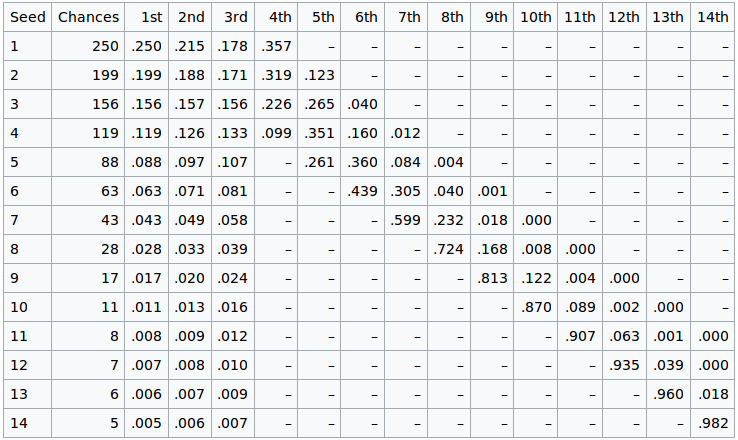
\includegraphics[scale=0.6]{../images/table.png} 
\end{center} \newpage

In order to better visualize these probabilities I created a couple plots displayed below. The first plot shows a given teams probability of receiving any of the first fourteen draft slots.
\begin{center}
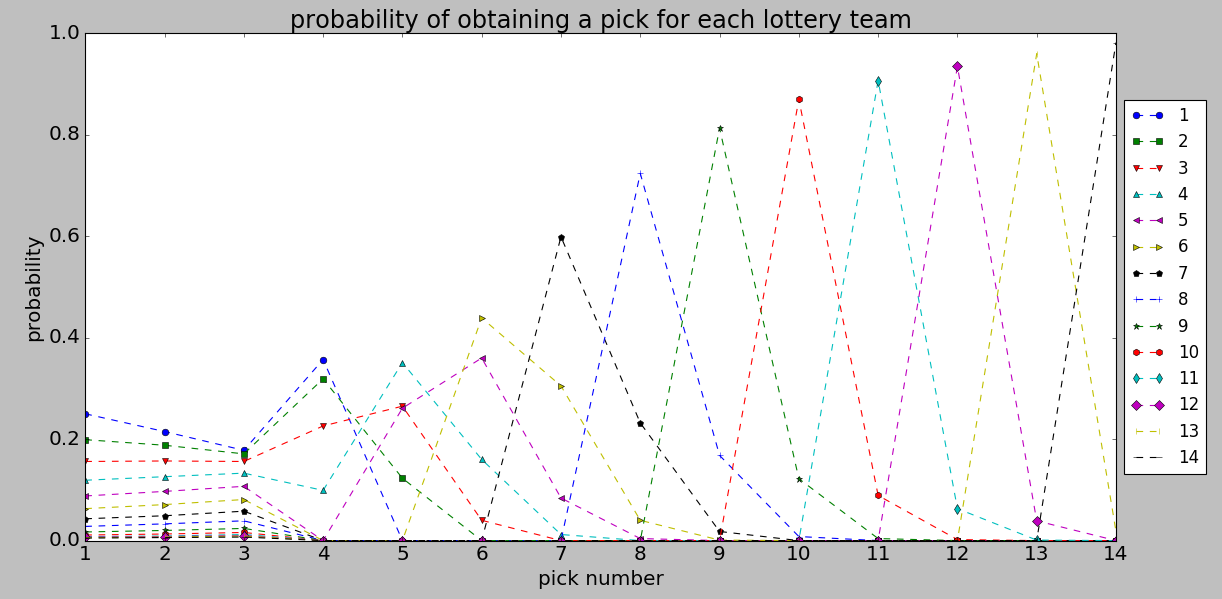
\includegraphics[scale=0.5]{../images/plot1.png} 
\end{center}

I found it interesting that as you move farther into the draft the teams are have more certainty around which pick they will be receiving. The next plot I created is quite similar, but instead of plotting the probability of a team receiving a pick, it displays the probability that a team will have picked by the $n^{th}$ slot of the draft. For example, team 1 will have .250 chance of having picked after round 1, and after round two they will have $.250 + .215 = .465$ chance of having picked.

\begin{center}
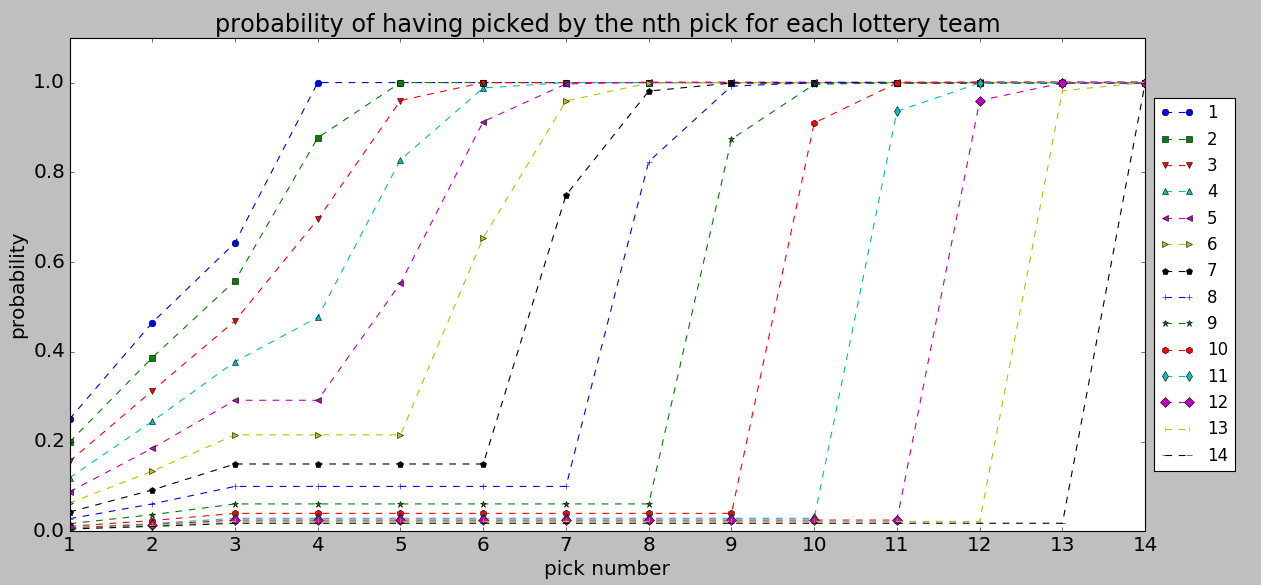
\includegraphics[scale=0.5]{../images/plot2.png} 
\end{center} \newpage

As expected, one team per round will reach a probability having picked of 1. This is due to the fact that the worst slot the rank 1 team can be assigned is fourth, and the result follows for the remaining teams. 

\section{Conclusions}
In a sport dominated by superstars, securing strong draft picks is hugely important for NBA teams. Though the process is complicated and long, it is nice to know that in a world where control is paramount, a little bit of randomness can turn expectation on its head. Thanks for reading. \\ \\ 
-dirty mike


\newpage
\begin{thebibliography}{99}

\bibitem{melissinos}
\url{https://en.wikipedia.org/wiki/NBA_draft_lottery}

\bibitem{Cyr}
\url{http://www.nba.com/news/draft/nba-draft-lottery-what-will-happen-2016/}

\bibitem{Wiki} 
\url{https://www.sbnation.com/nba/2017/4/13/15268144/nba-draft-lottery-odds-2017-lakers-celtics-suns}

\end{thebibliography}


\end{document}
